\chapter*{Results}

\section*{TCR repertoire preliminary analysis}

% One of the clinical characteristics of \covid-infected patients is lymphopenia or low lymphocyte counts in peripheral blood, specially affecting to T cells. The degree of lymphopenia correlates with disease severity, and it is usually associated with a pro-inflamatory cytokine storm \citep{lymphopeniaseverity}. It is hypothesized that the underlying causes of lymphopenia can be the pro-inflamatory cytokine levels, exhaustion of T cells upon COVID-19 infection and direct \covid-infection of T cells \citep{lymphopenia}.

One of the clinical characteristics of \covid-infected patients, lymphopenia, can be observed from a TCR repertoire analysis perspective. In TCR repertoire sequencing from a peripheral blood sample, both the number of nucleated cells and total T cells can be estimated by the amplification of reference gene primers. The fraction of T cells is significantly lower in convalescent individuals compared to vaccinated and placebo ($p = 2.5\cdot10^{-9}$ and $p = 5.6\cdot10^{-4}$, two-sided Wilcoxon rank-sum test) and no significant differences were observed between vaccinated and placebo subjects (Fig. \ref{fig:lymphopenia}a). Some convalescent patients \TCRB{} repertoires have a low Shannon diversity index (Fig. \ref{fig:lymphopenia}b), indicating that a few clones are expanded and possibly reflecting that these individuals had a recent adaptive immunity response, most likely to \covid{} infection.

%%% Sentence about lymphopenia affecting repertoire landscape???


\begin{figure}[!t]
	\centering
	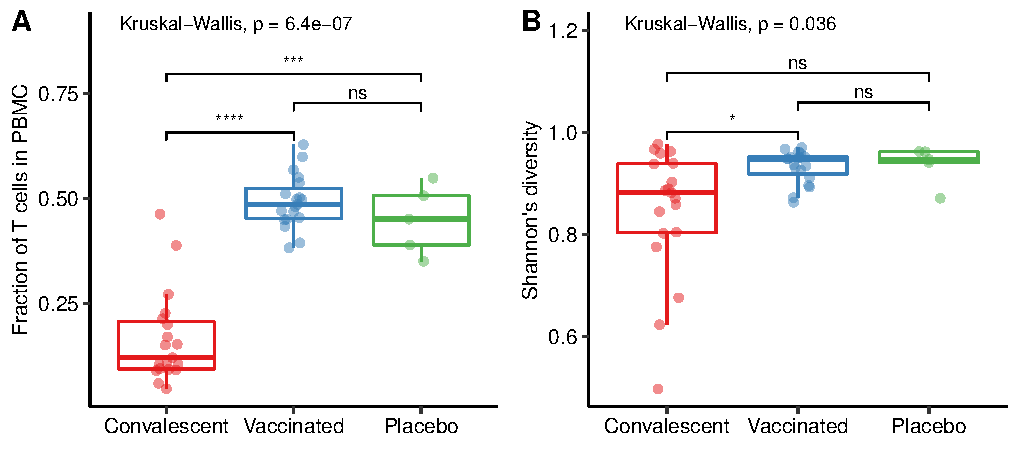
\includegraphics[width=0.7\textwidth,keepaspectratio]{figures/fig1.pdf}
	\caption{\textbf{TCR repertoire preliminary analysis. (a)} Fraction of T cells among peripheral blood mononuclear cells (PBMC). \textbf{(b)} Shannon diversity index. A value closer to 0 indicates the emergence of a few dominant clones, whereas it reaches its maximum when TCR frequencies are evenly distributed. Statistical significance was determined by two-sided Wilcoxon rank-sum tests. N = 43 independent samples (19 SARS-CoV-2 convalescent individuals, 19 Ad26.COV2.S vaccine recipients, 5 placebo recipients).}
	\label{fig:lymphopenia}
\end{figure}
%%% Pvalues asterisk equivalence?


\section*{Breadth and depth of \covid-specific T-cell response}

To evaluate the magnitude of the T-cell response to \covid{} after disease and vaccination, TCR repertoires of convalescent, vaccinated and placebo recipients individuals were annotated with CD8\textsuperscript{+} and CD4\textsuperscript{+} TCR datasets that had previously been determined to be \covid-specific and screened for enrichment compared to a background of healthy individuals repertoires in order to remove TCRs that may be unspecific (i.e. cross-reactive to common antigens) (See \nameref{chap:matmed}). Among the 43 repertoires analyzed there were 11,604,850 unique TCR sequences (V gene + CDR3 aminoacid sequence) of which only 284 were \covid-specific. Out of these annotated 284 TCRs, 51 were public (i.e. present in more than one individual).

Response to \covid{} spike and non-spike was measured in terms of breadth (unique TCR sequences) and depth (frequency of those TCRs). Both convalescent and vaccinated subjects have a higher spike-specific response compared to placebos in termns of breadth and depth (Fig. \ref{fig:bd}a). By contrast, breadth and depth of non-spike TCRs were significantly higher in convalescent individuals versus vaccinated and placebos, and there were no significant differences between the latter two (Fig. \ref{fig:bd}b), as expected because Ad26.COV2.S vaccine only carry the spike antigen.

\begin{figure}[t]
	\centering
	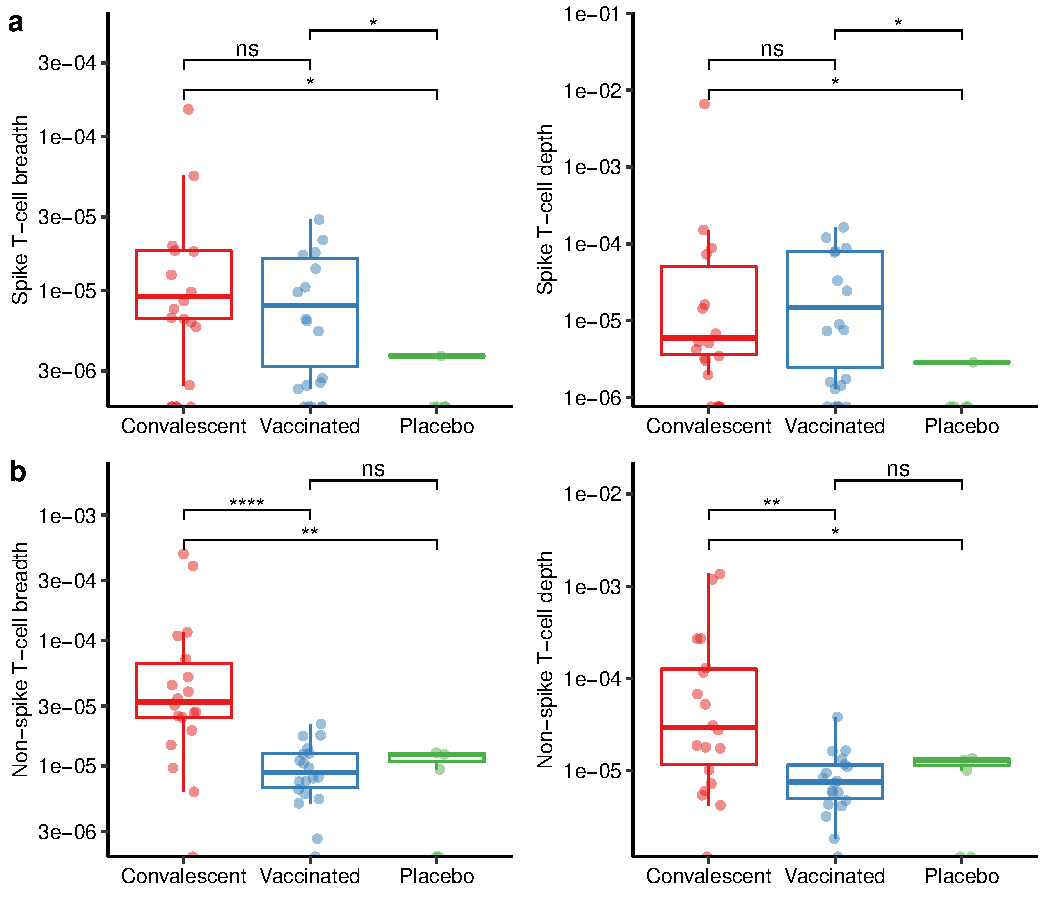
\includegraphics[width=0.7\textwidth,keepaspectratio]{figures/fig2.pdf}
	\caption{\textbf{\covid-specific \TCRB{} repertoire analysis. (a)} Spike-specific T-cell breadth and depth. \textbf{(b)} Non-spike-specific T-cell breadth and depth. Breadth is calculated as the fraction of unique TCR sequences specific to spike / non-spike proteins; depth is the relative frequency of those specific TCRs in the repertoire. Statistical significance was determined by two-sided Wilcoxon rank-sum tests. N = 43 independent samples (19 SARS-CoV-2 convalescent individuals, 19 Ad26.COV2.S vaccine recipients, 5 placebo recipients)}
	\label{fig:bd}
\end{figure}

\begin{figure}[t]
	\centering
	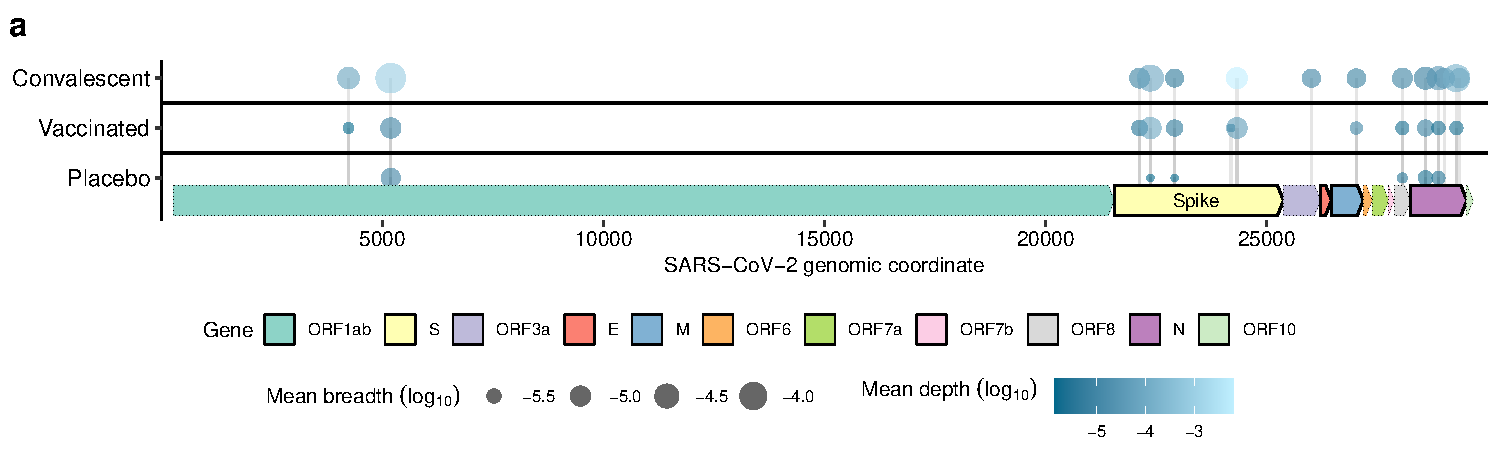
\includegraphics[width=\textwidth,keepaspectratio]{figures/hits.pdf}
	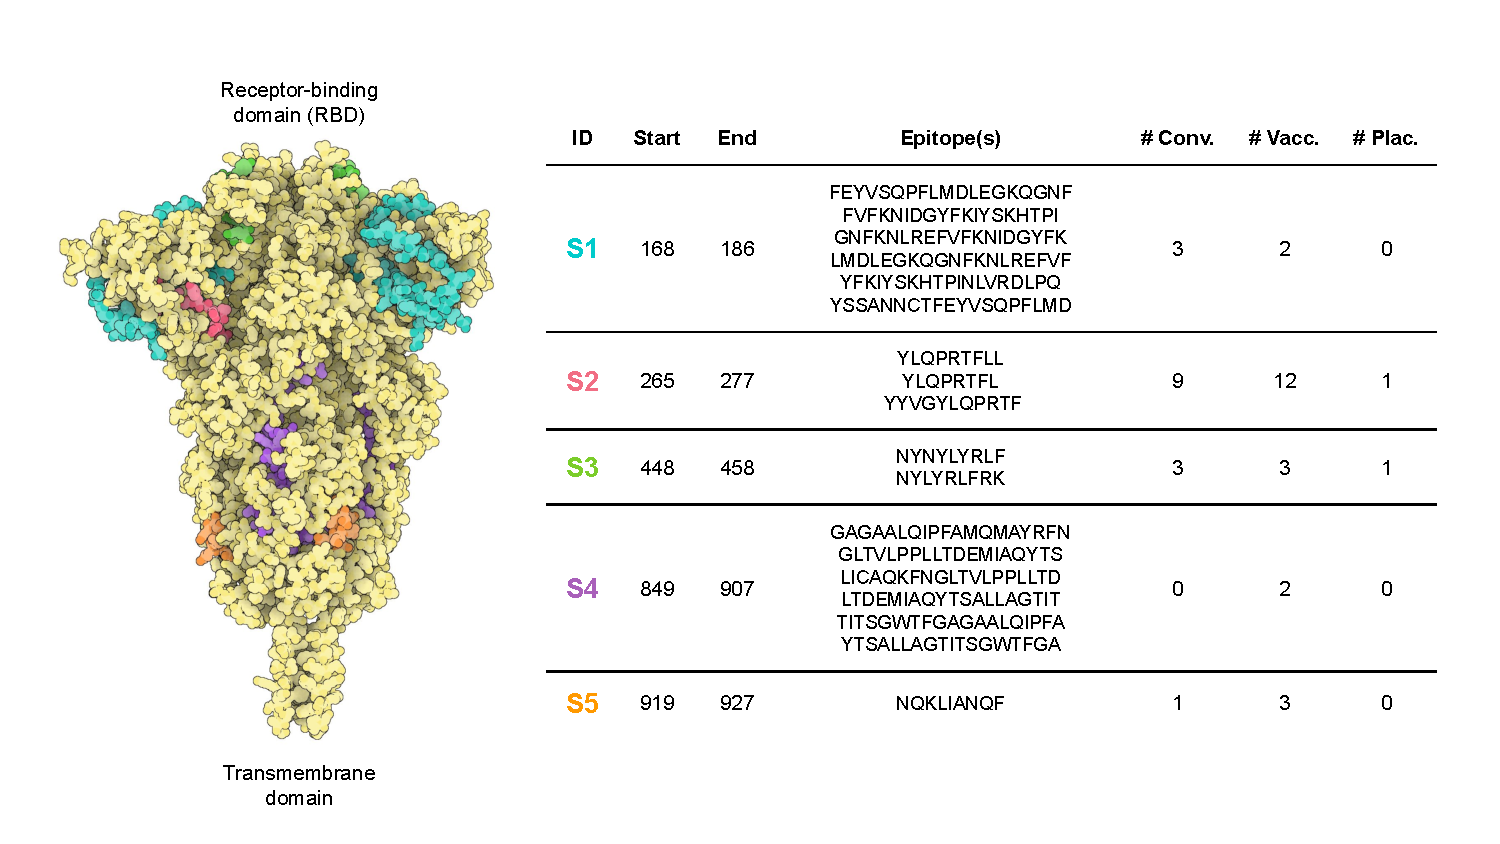
\includegraphics[width=0.7\textwidth,keepaspectratio]{figures/spike_w_table.pdf}
	\caption{\textbf{Epitopes recognized by T cells accross SARS-CoV-2 genome. (a)} Lollipop plot of the \TCRB{} \covid{} specificity in convalescent, vaccinated and placebo individuals accross the coronavirus genome. Size of the dots indicate the mean breadth accross all samples in a group and color scale indicates the mean depth of the response. Genes outlined with solid lines are structural (S, E, M and N), whereas dotted ones encode non-structural proteins. \textbf{(b)} Localization and characteristics of the 5 \covid{} spike epitopes recognized by TCRs in this study. Epitopes appear colored in the three monomers of a spike protein 3D representation (PDB: 6XR8, side view). Start, End: epitope protein coordinates (1-based); \# Conv., \# Vacc., \# Plac.: number of individuals in a group with TCRs specific to that epitope.}
	\label{fig:hits}
\end{figure}

An in-depth analysis of the genomic localization of \covid{} epitopes recognized by TCRs revealed that most of the T-cell immune response in convalescent individuals is directed towards structural proteins S and N (Fig. \ref{fig:hits}a). Although vaccinated subjects show some response to non-spike proteins, for most epitopes this signal is residual compared to the convalescent group and most likely due to unspecific annotations, since placebo recipients also show a minimal level of response. The localization of the 5 spike protein epitopes is shown in Fig. \ref{fig:hits}b. As opposed to B-cell epitopes, T-cell epitopes localization is not restricted to the protein surface since TCRs recognize antigens processed and presented in MHC molecules by human cells, and it shows in the spike protein 3D representation, where most of the epitopes are partially (S1, S3, S5) or completely (S2, S4) buried in the structue. S2 epitope is in fact the most widely recognized by convalescent (9/19) and vaccinated (12/19) individuals, and S4, the most hidden in the protein, is unrecognized by convalescent subjects and exclusively recognized by TCRs of 2 out of 19 vaccine recipients.




\section*{Network analysis}

The landscape of TCR repertoires is vast and complex. A simple antigen specificity annotation by V gene and CDR3 aminoacid sequence exact match, although informative and straightforward, can underestimate the magnitude of the T cell response. In order to capture the \covid-specific TCR repertoire architecture, graphs representing networks of similar TCRs were generated (Fig.\ref{fig:nets}a).

In addition, direct annotation with \covid-specific TCRs is not very precise, since there is some non-spike response in vaccine recipients, as well as response to some \covid{} epitopes in healthy placebo recipients (Figs. \ref{fig:bd}b, \ref{fig:hits}a). Network analysis can help identifying those nodes that truly are \covid-specific.

\textit{TO-DO - Main points:
- Vaccinated networks are richer than convalescent (more nodes and edges), reflecting lymphopenia
- Non-spike nodes have more authority in convalescent networks
- Non-spike nodes have more degree, loops and smaller distances in convalescent networks
- PCA with the mentioned variables effectively separates true covid-specific nodes
}

\textit{Figures in the making:
Fig 4b: covid similarity networks global metrics,
Fig 4c: authority of spike / non-spike nodes,
Fig 4d: degree, loops and distance histograms of spike / non-spike nodes,
Fig 4e: PCA with variables in 4c,d that separate true covid-specific nodes}


% \textcolor{lightgray}{\lipsum[1-2]}

\begin{figure}[t]
	\centering
	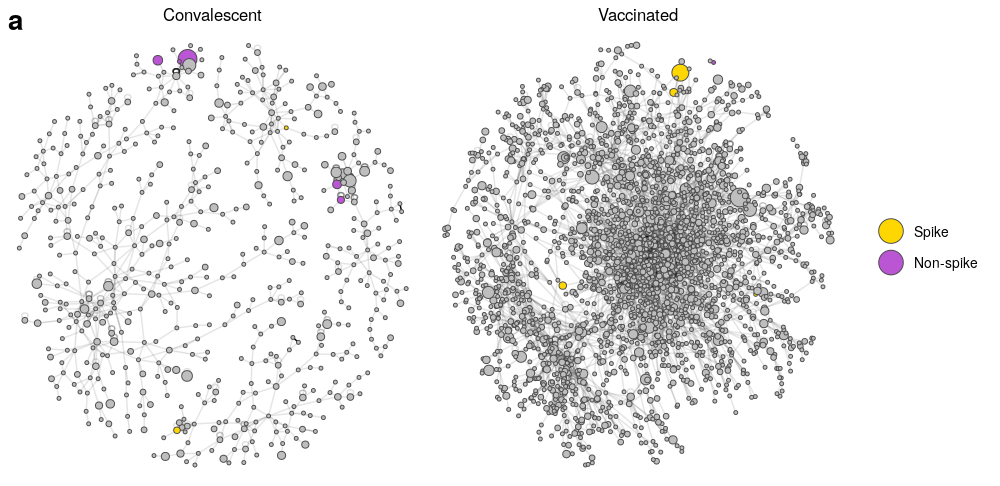
\includegraphics[width=0.8\textwidth,keepaspectratio]{figures/two_nets.png}
	\caption{\textbf{\covid-specific \TCRB{} similarity networks. (a)} \TCRB{} similarity networks where each node represents a unique V gene + CDR3 aminoacid sequence combination. Only \covid-specific nodes (colored) and the nodes in their components (gray) are shown for convalescent subject 18 and vaccinated subject 12. Two nodes are connected by and edge if their tcrdist3 distance is $\leq$ 12. Loops (self-edges that start and end at the same node) represent additional unique nucleotide sequences encoding the same V gene + amino acid sequence (i.e., convergence).}
	\label{fig:nets}
\end{figure}
